%!TEX root = ../thesis.tex

\chapter{Numerical Method}

This chapter fixes the finite-volume MUSCL--Hancock method used in Chapter~5.
Chapter~4 then varies precision, backend, compiler flags, and selected branch
rules around this fixed update.

\section{Finite-Volume Update}
% <<SECTION_1_BEGIN>>
For the ideal-gas Euler system the conserved state is
\(U=(\rho,\rho u,\rho v,E)^T\). In two dimensions it satisfies
\[
  U_t + F(U)_x + G(U)_y = 0,
\]
with physical fluxes
\[
  F(U)=
  \begin{pmatrix}
    \rho u\\ \rho u^2+p\\ \rho uv\\ u(E+p)
  \end{pmatrix},
  \qquad
  G(U)=
  \begin{pmatrix}
    \rho v\\ \rho uv\\ \rho v^2+p\\ v(E+p)
  \end{pmatrix}.
\]
On the Cartesian cell
\(C_{ij}=[x_{i-1/2},x_{i+1/2}]\times[y_{j-1/2},y_{j+1/2}]\), integrating over
\([t^n,t^{n+1}]\times C_{ij}\) gives
\[
\begin{aligned}
  &\int_{C_{ij}} U(x,y,t^{n+1})\,dx\,dy
  - \int_{C_{ij}} U(x,y,t^n)\,dx\,dy \\
  &\quad
  + \int_{t^n}^{t^{n+1}}\!\!\int_{y_{j-1/2}}^{y_{j+1/2}}
      \left[F(U(x_{i+1/2},y,t))-F(U(x_{i-1/2},y,t))\right]\,dy\,dt \\
  &\quad
  + \int_{t^n}^{t^{n+1}}\!\!\int_{x_{i-1/2}}^{x_{i+1/2}}
      \left[G(U(x,y_{j+1/2},t))-G(U(x,y_{j-1/2},t))\right]\,dx\,dt
  =0 .
\end{aligned}
\]
The discrete unknown is the cell average
\[
  \bar U_{ij}^{\,n}
  = \frac{1}{\Delta x\,\Delta y}
    \int_{C_{ij}} U(x,y,t^n)\,dx\,dy .
\]
The interface flux is the time- and face-averaged physical flux, approximated in
practice by a Riemann solver:
\[
  \widehat F_{i+1/2,j}^{\,n}
  =
  \frac{1}{\Delta t^n\,\Delta y}
  \int_{t^n}^{t^{n+1}}\!\!\int_{y_{j-1/2}}^{y_{j+1/2}}
  F(U(x_{i+1/2},y,t))\,dy\,dt ,
\]
with \(\widehat G_{i,j+1/2}^{\,n}\) defined analogously on horizontal faces.
Substitution gives the conservative flux-difference update
\begin{equation}\label{eq:fv-update}
  \bar U_{ij}^{\,n+1}
  =
  \bar U_{ij}^{\,n}
  - \frac{\Delta t^n}{\Delta x}
    \left(\widehat F_{i+1/2,j}^{\,n}
          -\widehat F_{i-1/2,j}^{\,n}\right)
  - \frac{\Delta t^n}{\Delta y}
    \left(\widehat G_{i,j+1/2}^{\,n}
          -\widehat G_{i,j-1/2}^{\,n}\right).
\end{equation}
A shared face therefore contributes equal and opposite fluxes to neighbouring
cells, so summing the update cancels all interior exchanges and leaves only
boundary fluxes. This cancellation is the finite-volume conservation mechanism
used below, following the standard treatments of \citet{toro2009} and
\citet{leveque_2002}. Equation~\ref{eq:fv-update} fixes the
two-direction notation; the implementation applies this conservative update
through alternating directional sweeps, described in Chapter~4. In two
dimensions each sweep is a one-dimensional conservative update using the current
cell averages; alternating the sweep order reduces a fixed ordering bias. The
scheme is therefore dimensionally split, not an unsplit method with transverse
flux corrections.
% <<SECTION_1_END>>

\section{MUSCL-Hancock Reconstruction and Predictor Step}
% <<SECTION_2_BEGIN>>
\paragraph{Slope limiting.}
The MUSCL-Hancock step uses a piecewise-linear reconstruction inside each cell,
followed by a half-time predictor before the Riemann solve. For conserved
component \(k\), define the one-sided jumps
\[
  \delta^- U_i^{(k)}=\bar U_i^{(k),n}-\bar U_{i-1}^{(k),n},
  \qquad
  \delta^+ U_i^{(k)}=\bar U_{i+1}^{(k),n}-\bar U_i^{(k),n}.
\]
The report path uses component-wise minbee, equivalently minmod-style, limiting:
\[
  \sigma_i^{(k)}
  =
  \operatorname{minmod}\!\left(\delta^- U_i^{(k)},\delta^+ U_i^{(k)}\right),
\]
where
\[
  \operatorname{minmod}(a,b)
  =
  \begin{cases}
    0, & ab\le 0,\\
    \operatorname{sgn}(a)\min\!\left(|a|,|b|\right), & ab>0 .
  \end{cases}
\]
In ratio form, where \(r_i^{(k)}=\delta^- U_i^{(k)}/\delta^+ U_i^{(k)}\) is
defined, this corresponds to
\[
  \sigma_i^{(k)}=\Phi(r_i^{(k)})\,\delta^+ U_i^{(k)},
  \qquad
  \Phi(r)=\max(0,\min(1,r)).
\]
This limiter keeps the slope zero across opposite-signed jumps and selects the
smaller monotone jump otherwise, reducing oscillations near discontinuities
while retaining second-order reconstruction in smooth monotone regions, following
\citet{vanleer_1979} and the presentation in \citet{toro2009}. Minbee is a diffusive TVD limiter, so small
perturbations may be damped more strongly than they would be with a less
diffusive limiter. Other limiters such as van~Leer or superbee exist in the
source tree, but Chapter~5 does not claim an isolated limiter-sensitivity
result.

\paragraph{Hancock predictor.}
The reconstructed states at the left and right faces of cell \(i\) are
\[
  U_{i,L}^{n}=\bar U_i^{n}-\frac12\sigma_i,
  \qquad
  U_{i,R}^{n}=\bar U_i^{n}+\frac12\sigma_i .
\]
They are then advanced through a local Hancock half step using the flux
difference across the reconstructed cell profile:
\[
  \bar U_{i,L}^{\,n+1/2}
  =
  U_{i,L}^{n}
  -\frac{\Delta t}{2\Delta x}
  \left[F(U_{i,R}^{n})-F(U_{i,L}^{n})\right],
\]
\[
  \bar U_{i,R}^{\,n+1/2}
  =
  U_{i,R}^{n}
  -\frac{\Delta t}{2\Delta x}
  \left[F(U_{i,R}^{n})-F(U_{i,L}^{n})\right].
\]
\paragraph{Riemann input.}
The Riemann problem at \(x_{i+1/2}\) is finally posed from neighbouring
predicted states,
\[
  U_{i+1/2}^{L}=\bar U_{i,R}^{\,n+1/2},
  \qquad
  U_{i+1/2}^{R}=\bar U_{i+1,L}^{\,n+1/2},
  \qquad
  \widehat F_{i+1/2}
  =
  \mathcal{R}\!\left(U_{i+1/2}^{L},U_{i+1/2}^{R}\right).
\]
The same construction applies in the \(y\)-direction with \(G\), \(\Delta y\),
and bottom/top reconstructed states.
% <<SECTION_2_END>>

\section{HLLC and Rusanov Fluxes}
% <<SECTION_3_BEGIN>>
At a vertical interface the predictor supplies left and right states \(U_L\) and
\(U_R\), so the local problem is the one-dimensional Riemann problem
\[
  U_{\mathrm{RP}}(x,0)=
  \begin{cases}
    U_L, & x<0,\\
    U_R, & x>0 .
  \end{cases}
\]
The report's main validation flux is HLLC. In the construction introduced by
\citet{toro_spruce_speares_1994} and presented in \citet{toro2009}, this flux
approximates the fan by left, contact, and right waves with speeds \(S_L\),
\(S_\ast\), and \(S_R\). In the implemented Davis estimate,
\[
  S_L=\min(u_L-a_L,u_R-a_R), \qquad
  S_R=\max(u_L+a_L,u_R+a_R),
\]
and
\[
  S_\ast =
  \frac{p_R-p_L+\rho_L u_L(S_L-u_L)-\rho_R u_R(S_R-u_R)}
       {\rho_L(S_L-u_L)-\rho_R(S_R-u_R)} .
\]
\begin{figure}[htbp]
\centering
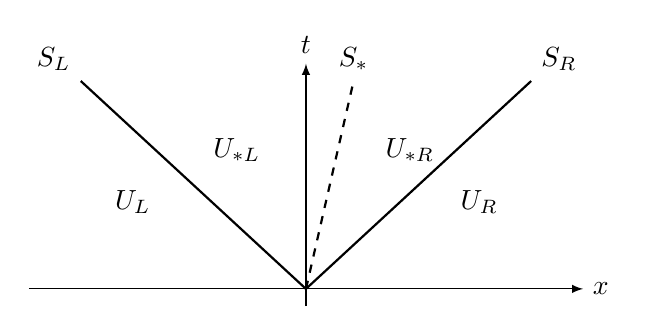
\begin{tikzpicture}[>=latex,scale=1.1]
  \draw[->] (-3.2,0) -- (3.2,0) node[right] {$x$};
  \draw[->] (0,-0.2) -- (0,2.6) node[above] {$t$};
  \draw[thick] (0,0) -- (-2.6,2.4) node[above left] {$S_L$};
  \draw[thick] (0,0) -- (2.6,2.4)  node[above right] {$S_R$};
  \draw[thick,dashed] (0,0) -- (0.55,2.4) node[above] {$S_\ast$};
  \node at (-2.0,1.0) {$U_L$};
  \node at (-0.8,1.6) {$U_{\ast L}$};
  \node at ( 1.2,1.6) {$U_{\ast R}$};
  \node at ( 2.0,1.0) {$U_R$};
\end{tikzpicture}
\caption{Three-wave HLLC structure at an interface: left and right acoustic
waves with speeds \(S_L\) and \(S_R\) bound two star states \(U_{\ast L}\) and
\(U_{\ast R}\), separated by a contact discontinuity moving at \(S_\ast\). The
sign of these three speeds selects the interface flux in HLLC.}
\label{fig:hllc-fan}
\end{figure}

The approximate solution sampled at \(\xi=x/t\) is
\[
  \tilde U(\xi)=
  \begin{cases}
    U_L, & \xi<S_L,\\
    U_{\ast L}, & S_L<\xi<S_\ast,\\
    U_{\ast R}, & S_\ast<\xi<S_R,\\
    U_R, & S_R<\xi .
  \end{cases}
\]
The corresponding interface flux is selected by the sign of the wave speeds:
\[
  \widehat F_{\mathrm{HLLC}}=
  \begin{cases}
    F_L, & 0\le S_L,\\
    F_{\ast L}, & S_L\le 0 \le S_\ast,\\
    F_{\ast R}, & S_\ast\le 0 \le S_R,\\
    F_R, & S_R\le 0 .
  \end{cases}
\]
For \(K\in\{L,R\}\), the star-region flux is written as
\[
  F_{\ast K}=F_K+S_K\left(U_{\ast K}-U_K\right),
\]
where \(U_{\ast K}\) is obtained from the Rankine--Hugoniot jump conditions
across \(S_K\) and may be written in closed form as
\[
  U_{\ast K}
  =
  \rho_K\,\frac{S_K-u_K}{S_K-S_\ast}
  \begin{pmatrix}
    1\\[2pt]
    S_\ast\\[2pt]
    v_K\\[2pt]
    \dfrac{E_K}{\rho_K}
    +(S_\ast-u_K)\!\left[S_\ast+\dfrac{p_K}{\rho_K(S_K-u_K)}\right]
  \end{pmatrix},
\]
with the contact pressure
\(p_\ast=p_K+\rho_K(S_K-u_K)(S_\ast-u_K)\) equal on both sides of the contact.
This is the part of HLLC that restores the contact wave missing from the
two-wave HLL approximation discussed by \citet{toro_spruce_speares_1994} and
\citet{toro2009}. The exact choice of strict or non-strict
inequality at zero is a precision-sensitive implementation decision and is
discussed separately in Section~\ref{sec:precision-sensitive-decisions}.

Rusanov is used later as a more diffusive comparator and method variation, not
as the main validation method. It replaces the contact-resolving HLLC structure
by a centred flux plus scalar dissipation,
\[
  \widehat F_{\mathrm{Rus}}
  =
  \frac12\left(F_L+F_R\right)
  -\frac12 S_{\max}\left(U_R-U_L\right),
  \qquad
  S_{\max}=\max\left(|u_L|+a_L,\ |u_R|+a_R\right).
\]
This form is useful for comparison because it has a single local signal-speed
penalty and no contact-wave branch, but its stronger numerical diffusion can
smear contacts and shear layers relative to HLLC, as expected for the HLL family
introduced by \citet{harten_lax_vanleer_1983} and described by
\citet{toro2009}.
% <<SECTION_3_END>>

\section{Stability, Limiting, and Positivity}
% <<SECTION_4_BEGIN>>
Stability is controlled by nondimensional Courant numbers rather than by the
time step alone. For the Euler equations the relevant one-cell signal speeds are
the acoustic bounds in each coordinate direction, so a local update can be
described by
\[
  \nu_{x,ij}
  =
  \frac{\Delta t}{\Delta x}\left(|u_{ij}|+c_{ij}\right),
  \qquad
  \nu_{y,ij}
  =
  \frac{\Delta t}{\Delta y}\left(|v_{ij}|+c_{ij}\right),
\]
where \(c_{ij}\) is the sound speed. In the implemented update the time step is
selected globally from the local wave speeds,
\[
  \Delta t^{n}
  =
  C_{\mathrm{CFL}}\,
  \min_{ij}\!\left(
    \frac{\Delta x}{|u_{ij}|+c_{ij}},\
    \frac{\Delta y}{|v_{ij}|+c_{ij}}
  \right),
  \qquad
  0<C_{\mathrm{CFL}}\le 1,
\]
so that \(\max_{ij}\max(\nu_{x,ij},\nu_{y,ij})\le C_{\mathrm{CFL}}\). The
implemented update is dimensionally split: Equation~\ref{eq:fv-update} is
applied as successive one-dimensional sweeps in \(x\) and \(y\). The working
role of \(C_{\mathrm{CFL}}\) is therefore a safety factor on the local acoustic
wave-speed restriction, not a universal stability constant
\citep{toro2009,leveque_2002}.

For a scalar monotone first-order scheme, a TVD argument gives a direct
Courant-number restriction. MUSCL-Hancock uses second-order reconstruction and a
predictor step, then relies on limiting to suppress new oscillations near
nonsmooth data. The limiter makes the reconstruction nonlinear, so the local
order is not uniform across the grid. In smooth monotone regions the
piecewise-linear data and Hancock predictor give the expected second-order
truncation behaviour. At extrema, shocks, contacts, and rarefaction edges the
minbee/minmod-type limiter can set or reduce the slope, moving the local update
towards a first-order Godunov step \citep{vanleer_1979,toro2009}.

The same restriction is also tied to physical admissibility. The primitive
conversion requires
\[
  \rho > 0,
  \qquad
  p=(\gamma-1)\left(E-\frac12\rho(u^2+v^2)\right)>0 .
\]
Large Courant numbers, strong waves, or near-vacuum states can produce predicted
or updated states outside this admissible set even when the conservative update
is algebraically well defined. HLLC wave-speed estimates and limiter decisions
therefore act together with the CFL choice: they determine not only linear
stability, but also whether the intermediate states used in the Riemann solve
remain physically meaningful. No general positivity proof is claimed here; the
CFL and limiter choices are treated as part of the controlled numerical method.
% <<SECTION_4_END>>

\section{Precision-Sensitive Decision Points}
\label{sec:precision-sensitive-decisions}
% <<SECTION_5_BEGIN>>
\paragraph{Rounding model.}
A useful local model for the floating-point part of the method is the standard
one-operation rounding model
\[
  \operatorname{fl}(a \mathbin{\mathrm{op}} b)
  =
  (a \mathbin{\mathrm{op}} b)(1+\delta),
  \qquad |\delta|\le u ,
\]
for a basic arithmetic operation under round-to-nearest-even IEEE\,754 semantics,
away from overflow, underflow, and exceptional cases
\citep{ieee754_2019,goldberg_1991,higham_2002}. A flux
evaluation is then a composed map rather than one rounded operation: primitive
recovery, sound-speed evaluation, wave-speed estimates, star-state construction,
and flux differences each introduce small perturbations. If the final update
were a smooth function of the cell averages only, this would mainly be an error
propagation question. HLLC also contains comparisons, so rounded real numbers
can change which algebraic formula is sampled at an interface.

\paragraph{Branch sensitivity.}
For HLLC, the branch decision is made from computed estimates
\(\widehat S_L,\widehat S_\ast,\widehat S_R\), not exact wave speeds. Thus the
logical test
\[
  S_L \le 0 \le S_\ast
  \qquad\hbox{or}\qquad
  S_L < 0 < S_\ast
\]
is sensitive when one of the speeds is close to zero. The two versions differ
only on equality in exact arithmetic, but equality and near-equality are not
innocent in a rounded implementation: the computed sign of \(\widehat S_\ast\)
is the result of a quotient. Writing
\[
  S_\ast=\frac{N_\ast}{D_\ast}, \qquad
  D_\ast=\rho_L(S_L-u_L)-\rho_R(S_R-u_R),
\]
shows the possible conditioning issue. A first-order perturbation gives
\[
  \frac{\Delta S_\ast}{S_\ast}
  \approx
  \frac{\Delta N_\ast}{N_\ast}
  -
  \frac{\Delta D_\ast}{D_\ast},
\]
when the terms are non-zero. This does not prove that the reported tests contain
large \(S_\ast\) errors. It identifies a mechanism: cancellation or a small
denominator can amplify rounded changes in the wave-speed estimate, and the
amplified value may then enter a discontinuous branch selection \citep{toro2009}.

\paragraph{Measured versus concept-only axes.}
The controlled axes in this report are therefore separated from conceptual
sources of sensitivity. The HLLC branch-rule comparison is controlled by
\texttt{RIEMANN\_STRICT\_INEQUALITY} and tests \(<\) rather than \(\le\) in the
wave-speed branch. The CPU compiler-flag rows compare gcc \texttt{-O2},
\texttt{-O3}, and \texttt{-Ofast} with fast-math, while the CUDA
strict-versus-fast probe in Chapter~5 separately tests the build-control effect
of disabling \texttt{STRICT\_IEEE} and enabling \texttt{FAST\_MATH}. These flags
can change expression evaluation through reassociation, fused operations,
flush-to-zero behaviour, or approximate division and square root; they do not
change the finite-volume formula. The fp32 axis changes the unit roundoff and
exponent range relative to fp64, using real binary32 runs rather than a
surrogate precision. By contrast, exact-solver stopping tolerances, alternative
limiter choices, and general parallel reduction ordering are discussed only as
possible sensitivity mechanisms unless an isolated experiment is shown for them.

\begin{table}[htbp]
\centering
\small
\begin{tabularx}{\textwidth}{@{}l>{\raggedright\arraybackslash}X>{\raggedright\arraybackslash}X@{}}
\toprule
Method component & Role in the update & Precision-sensitive point \\
\midrule
Limited reconstruction & Builds left/right states for the Hancock predictor &
Limiter branches can change local order near extrema or shocks. \\
Hancock predictor & Evolves reconstructed states by a half step before the
Riemann solve & Flux differences combine rounded primitive recovery and
energy terms. \\
HLLC flux & Selects the contact-resolving interface flux & Wave-speed tests
near zero expose the \(<\) versus \(\le\) branch rule. \\
CFL selection & Sets the explicit time step from acoustic signal speeds &
Global maxima and final-time clipping can differ across precision or evaluation
order. \\
Rusanov flux & Provides a deliberately more diffusive comparator & It removes
the contact branch, so differences from HLLC are method variation rather than
reproducibility drift. \\
\bottomrule
\end{tabularx}
\caption{Numerical-method components that matter for the precision and hardware
experiments.}
\label{tab:method-decision-points}
\end{table}
% <<SECTION_5_END>>

\section{Extension to Ideal MHD}
% <<SECTION_6_BEGIN>>
The Euler system used in Report 1 is the hydrodynamic limit of the later
ideal-MHD problem. The MHD conserved state adds magnetic-field components to
density, momentum, and energy, and the fluxes add magnetic pressure, magnetic
tension, and induction terms. This changes the characteristic structure: the
Riemann fan contains fast, Alfven, slow, and contact families rather than only
acoustic waves and a contact. The magnetic field must also satisfy
\[
  \nabla\cdot B = 0,
\]
at the continuous level. A finite-volume discretisation does not preserve this
constraint automatically, so choices such as the divergence cleaning of
\citet{dedner_2002} or the constrained transport of
\citet{evans_hawley_1988} become part of the
numerical method rather than optional diagnostics.

For this report, these MHD equations define the project context only. The
validated evidence in later chapters is for Euler tests, where exact or
high-resolution reference solutions and matched precision/device comparisons are
available. Extending the same evidence chain to ideal MHD requires separate
validation of the additional waves, magnetic-energy coupling, and discrete
divergence control; a GPU-accelerated MUSCL-Hancock baseline of the form
intended for Report~2 is described by \citet{bard_dorelli_2014}.
% <<SECTION_6_END>>
